% Volume III, Chapter 5: the gamma factor, the primes and the spline lemma. Sources: misc/reviews/nick-volume3/vol3/ch3_gamma_primes.tex (lines per misc/vol3/STRUCTURE.md, Chapter 5), referee reports U03 (M1 to M6) and V3C (ch3 part). 17 Nov 2026.
\label{g:ch:gammaprimes}

Nakamura's signed L\'evy measure of $\log\xi$ is one measure $\mu$ on $(0,\infty)$ (Chapter~\ref{n:ch:nakamura}, Proposition~\ref{n:prop:oneline}), with
\begin{gather*}
\mu=\sum_{n\ge2}\Lambda(n)\,\delta_{\log n}+\frac{\mathrm dx}{1-e^{-2x}}-\mathrm dx-e^x\mathrm dx,\\
(\log\xi)''(s)=\int_0^\infty x\,e^{-sx}\mu(\mathrm dx)\quad(\Re s>1),
\end{gather*}
where $\xi(s)=\frac12s(s-1)\Gamma_{\mathbb R}(s)\zeta(s)$ and $\Gamma_{\mathbb R}(s)=\pi^{-s/2}\Gamma(s/2)$. The four terms come from the primes, the gamma factor, the factor $s$ and the factor $s-1$. This chapter reads the gamma factor and the primes side by side. It is built on an unrefereed note of Polson (November 2026). Status words follow the book: the identities of Sections~\ref{g:sec:ledger} to \ref{g:sec:reg} and \ref{g:sec:splinelemma} to \ref{g:sec:fr} are proved, the table values are computed, and the equivalences are conditional only where a hypothesis is named. The Schoenberg criterion and the Pólya frequency ladder are in Chapter~\ref{chap:polyazeros} of Volume II (Proposition~\ref{pol:prop:pf}, Problem~\ref{pol:op:pf2}, Theorem~\ref{pol:thm:pf2}); the sections on splines use them.

\section{The ledger}\label{g:sec:ledger}

\begin{lemma}[Ledger rule]\label{g:lem:ledger}
For $a\in\mathbb C$ and $\Re s>\Re a$,
\[
\frac{\mathrm d^2}{\mathrm ds^2}\log(s-a)=-\frac{1}{(s-a)^2}=-\int_0^\infty x\,e^{-sx}\,e^{ax}\mathrm dx .
\]
Hence, if $(\log f)''(s)=\int_0^\infty xe^{-sx}\mu_f(\mathrm dx)$ on a right half plane, a zero of $f$ at $a$ contributes $-e^{ax}\mathrm dx$ to $\mu_f$ and a pole contributes $+e^{ax}\mathrm dx$.
\end{lemma}

\begin{proof}
$\int_0^\infty xe^{-(s-a)x}\mathrm dx=(s-a)^{-2}$ for $\Re(s-a)>0$.
\end{proof}

A zero far to the left is damped ($e^{-2kx}$ for the trivial zeros), a zero on the critical line oscillates with amplitude $e^{x/2}$, and the pole of $\zeta$ at $s=1$ grows like $e^x$. At level $\sigma$ the L\'evy measure is $e^{-\sigma x}\mu(\mathrm dx)/x$, so each exponential $e^{ax}$ becomes $e^{(a-\sigma)x}/x$. Table~\ref{g:tab:ledger} lists the contributions factor by factor.

\begin{table}[t]
\centering
\small
\begin{tabular}{llll}
\toprule
factor & zeros and poles & contribution to $\mu$ & sign\\
\midrule
$s$ & zero at $0$ & $-\mathrm dx$ & negative\\
$s-1$ & zero at $1$ & $-e^x\mathrm dx$ & negative\\
$\Gamma_{\mathbb R}(s)$ & poles at $-2k$, $k\ge0$ & $\sum_{k\ge0}e^{-2kx}\mathrm dx=\frac{\mathrm dx}{1-e^{-2x}}$ & positive\\
$\zeta(s)$ & Euler product & $\sum_n\Lambda(n)\delta_{\log n}$ & positive\\
\midrule
$\xi(s)$ & zeros $\rho$ only & $-\sum_\rho e^{\rho x}\mathrm dx$ & oscillating\\
\bottomrule
\end{tabular}
\caption{The ledger for $\xi$.}\label{g:tab:ledger}
\end{table}

\begin{proposition}\label{g:prop:ledger}
For $\Re s>1$,
\begin{multline}\label{g:eq:ledger}
\int_0^\infty xe^{-sx}\Big[\sum_n\Lambda(n)\delta_{\log n}+\frac{\mathrm dx}{1-e^{-2x}}-\mathrm dx-e^x\mathrm dx\Big]\\
=-\sum_\rho\int_0^\infty xe^{-sx}e^{\rho x}\mathrm dx,
\end{multline}
the sum over $\rho$ taken with $\rho$ and $\bar\rho$ paired. The identity of the two measures, $\sum_n\Lambda(n)\delta_{\log n}+\frac{\mathrm dx}{1-e^{-2x}}-\mathrm dx-e^x\mathrm dx=-\sum_\rho e^{\rho x}\mathrm dx$, holds as an identity of distributions on $(0,\infty)$ (the sum over $\rho$ is not a measure).
\end{proposition}

\begin{proof}
The left side is $(\log\xi)''(s)$ by Proposition~\ref{n:prop:oneline}, each row of Table~\ref{g:tab:ledger} being Lemma~\ref{g:lem:ledger} applied to the zeros and poles of that factor (for $\zeta$, directly from $-\zeta'/\zeta=\sum\Lambda(n)n^{-s}$). The right side is $(\log\xi)''(s)=-\sum_\rho(s-\rho)^{-2}$ from the Hadamard product, which converges absolutely because $\sum|s-\rho|^{-2}<\infty$; each term is Lemma~\ref{g:lem:ledger} with $a=\rho$, valid since $\Re\rho<1<\Re s$.
\end{proof}

Integrating \eqref{g:eq:ledger} once, on the scale $X=e^x>1$, gives the Riemann von Mangoldt explicit formula
\begin{equation}\label{g:eq:explicit}
\psi_0(X)=X-\sum_\rho\frac{X^\rho}{\rho}-\log2\pi-\tfrac12\log\big(1-X^{-2}\big),
\end{equation}
where $\psi_0$ is Chebyshev's function with the midpoint convention at jumps and the zero sum is taken symmetrically in the height. The constant $-\log 2\pi$ is not produced by the integration and is fixed independently. The term $-\frac12\log(1-X^{-2})=\sum_{k\ge1}X^{-2k}/2k$ is the share of the gamma factor that survives the factor $s$. Figure~\ref{g:fig:explicit} shows both sides.

\begin{figure}[t]
\centering
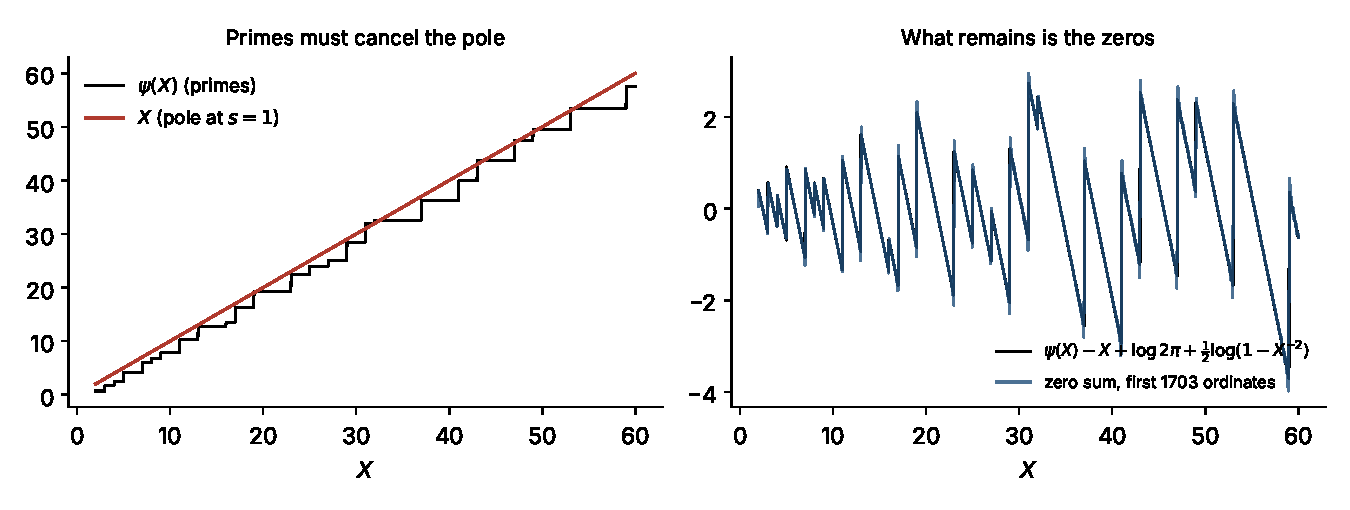
\includegraphics[width=\textwidth]{fig/v3/fig_explicit.pdf}
% UNVERIFIED: figure not checked by either referee (the 1703 and 2200 in the caption are verified)
\caption{Left: the primes, through $\psi(X)$, track the pole term $X$. Right: after the pole and the gamma terms are removed, what remains is the zero sum, here over the first $1703$ ordinates (up to height $2200$).}
\label{g:fig:explicit}
\end{figure}

\begin{remark}[Three cancellations]\label{g:rem:four}
The ledger is a bookkeeping device, and its three cancellations are readings of Table~\ref{g:tab:ledger}, not separate theorems. First, the factor $s$ cancels the pole of $\Gamma(s/2)$ at $s=0$ exactly: $-\mathrm dx+e^{0\cdot x}\mathrm dx=0$, which is $s\,\Gamma(s/2)=2\,\Gamma(s/2+1)$; what survives of the gamma row is $\sum_{k\ge1}e^{-2kx}\mathrm dx=\mathrm dx/(e^{2x}-1)$. Second, the poles of $\Gamma(s/2)$ at $-2k$, $k\ge1$, cancel the trivial zeros of $\zeta$ exactly: Lemma~\ref{g:lem:ledger} applied to $\zeta$ alone puts $-\sum_{k\ge1}e^{-2kx}\mathrm dx$ into the prime measure. Third, the pole of $\zeta$ is matched by the primes on average: the comb $\sum\Lambda(n)\delta_{\log n}$ has mean density $e^x$ on the logarithmic scale, which is the prime number theorem $\psi(X)\sim X$ and is equivalent to the absence of zeros on $\Re s=1$. What remains is $-\sum_\rho e^{\rho x}\mathrm dx$, a distribution whose exponents have real parts $\beta=\Re\rho$; RH says that every exponent has real part $\frac12$.\end{remark}

\section{The ledger with random variables}\label{g:sec:rv}

For $\sigma>1$ and $w\ge0$, each local factor is a Laplace transform.

\begin{proposition}\label{g:prop:rv}
Let $G_p$ be independent with $\mathbb P(G_p=m)=(1-p^{-\sigma})p^{-m\sigma}$, $m\ge0$, and let $E_k\sim\mathrm{Exp}(\sigma+2k)$, $k\ge0$, be independent exponential variables with the indicated rates. Then
\begin{align*}
\frac{\zeta(\sigma+w)}{\zeta(\sigma)}&=\mathbb E\,e^{-wZ},\qquad Z=\sum_pG_p\log p,\\
\frac{\Gamma_{\mathbb R}(\sigma+w)}{\Gamma_{\mathbb R}(\sigma)}\,e^{-wc_\Gamma}&=\prod_{k\ge0}\frac{\sigma+2k}{\sigma+2k+w}\,e^{w/(\sigma+2k)}\\
&=\mathbb E\,e^{-w(Y-\mathbb EY)},\qquad Y=\sum_{k\ge0}E_k,
\end{align*}
with $c_\Gamma=\Gamma_{\mathbb R}'(\sigma)/\Gamma_{\mathbb R}(\sigma)=-\frac12\log\pi+\frac12\psi(\sigma/2)$, where $Y-\mathbb EY$ is the almost sure limit of the centred partial sums. Further, $\frac{\sigma+w}{\sigma}=1/\mathbb Ee^{-wE_\sigma}$ and $\frac{\sigma-1+w}{\sigma-1}=1/\mathbb Ee^{-wE'}$ with $E_\sigma\sim\mathrm{Exp}(\sigma)$ and $E'\sim\mathrm{Exp}(\sigma-1)$.
\end{proposition}

\begin{proof}
The Euler product gives the first line, each factor $(1-p^{-\sigma})/(1-p^{-\sigma-w})$ being the Laplace transform of $G_p\log p$. For the second, the Weierstrass product $\Gamma(z+v)/\Gamma(z)=e^{v\psi(z)}\prod_{k\ge0}\frac{z+k}{z+k+v}e^{v/(z+k)}$ with $z=\sigma/2$, $v=w/2$ gives the product, and $\frac{\sigma+2k}{\sigma+2k+w}=\mathbb Ee^{-wE_k}$. The centred sum converges almost surely since $\sum\mathrm{Var}\,E_k=\sum(\sigma+2k)^{-2}<\infty$. The last statement is the Laplace transform of an exponential law.
\end{proof}

The exponential variables $E_k$ with $k\ge1$ are the trivial zeros, read as laws, and $E_0$ cancels the factor $s$. The primes contain an exponential variable of rate $\sigma-1$ only at the level of exponents: with $Z$ as above,
\[
\log\mathbb Ee^{-wZ}=\log\mathbb Ee^{-wE'}+\log\frac{(\sigma-1+w)\,\zeta(\sigma+w)}{(\sigma-1)\,\zeta(\sigma)},
\]
and the last logarithm has the signed L\'evy measure $e^{-\sigma x}\mathrm d\big(\psi(e^x)-e^x\big)/x$, while $E'$ has L\'evy measure $e^{-(\sigma-1)x}\mathrm dx/x$, the prime number theorem density. The remaining factor is not the Laplace transform of any random variable: it grows linearly in $w$ as $w\to\infty$, because $\zeta(\sigma+w)\to1$, while the transform of a variable $R\ge0$ is at most $1$, and grows at least exponentially if $\mathbb P(R<0)>0$. So the "prime remainder" is a signed measure and not a law. What survives the exact cancellations is Nakamura's measure $-\sum_\rho e^{(\rho-\sigma)x}/x$ (Remark~\ref{g:rem:four}).

\section{Finite primes and the infinite prime}\label{g:sec:local}

Applying Lemma~\ref{g:lem:ledger} to each local factor separately puts the gamma factor on the same footing as the Euler factors, as in Tate's thesis \cite{Tate67}, where the completed zeta function is $\Gamma_{\mathbb R}(s)\zeta(s)=\prod_{v\le\infty}L_v(s)$ with $L_\infty=\Gamma_{\mathbb R}$.

\begin{proposition}\label{g:prop:local}
\begin{enumerate}
\item $L_p(s)=(1-p^{-s})^{-1}$ has poles at $s=2\pi ik/\log p$, $k\in\mathbb Z$. Its measure is, by the Poisson summation formula, $\sum_{k\in\mathbb Z}e^{2\pi ikx/\log p}=\log p\sum_{m\in\mathbb Z}\delta_{m\log p}$, which on $(0,\infty)$ is the comb $\sum_{m\ge1}\log p\,\delta_{m\log p}$, the prime powers of $p$ in $\sum\Lambda(n)\delta_{\log n}$.
\item $L_\infty(s)=\Gamma_{\mathbb R}(s)$ has poles at $s=-2k$, $k\ge0$. Its measure is $\sum_{k\ge0}e^{-2kx}\mathrm dx$, a smooth density.
\end{enumerate}
The pole sums are conditionally convergent, and the identities hold as distributions.
\end{proposition}

\begin{proof}
For 1, $(\log L_p)''(s)=\sum_{m\ge1}(\log p)\,m\log p\;p^{-ms}=\allowbreak\int_0^\infty xe^{-sx}\allowbreak\sum_{m\ge1}\allowbreak\log p\,\delta_{m\log p}(\mathrm dx)$ directly, and the Poisson summation formula identifies this comb with the sum of the exponentials attached to the poles by Lemma~\ref{g:lem:ledger}. For 2 use $\frac14\psi'(s/2)=\int_0^\infty xe^{-sx}(1-e^{-2x})^{-1}\mathrm dx$.
\end{proof}

A finite prime has its poles spread vertically, on $\Re s=0$, and its measure is a discrete comb. The infinite prime has its poles spread horizontally, on the real axis, and its measure is smooth.

\section{Product forms of the gamma function}\label{g:sec:euler}

\subsection{Over the poles: Weierstrass and Gauss}

The classical products are
\[
\frac1{\Gamma(z)}=z\,e^{\gamma_Ez}\prod_{k\ge1}\Big(1+\frac zk\Big)e^{-z/k},\qquad
\Gamma(z)=\lim_{n\to\infty}\frac{n!\,n^z}{z(z+1)\cdots(z+n)} .
\]
Each factor $(1+z/k)^{-1}$ is the Laplace transform of an exponential law, the continuous analogue of the geometric law $\frac{1-p^{-\sigma}}{1-p^{-\sigma-w}}$ of a prime (Proposition~\ref{g:prop:rv}). The product diverges without compensation, and Gauss's factor $n^z=e^{z\log n}$ plays the role that Mertens's theorem $\prod_{p\le x}(1-p^{-1})^{-1}\sim e^{\gamma_E}\log x$ plays for the primes.

\subsection{Regularised products}

For a sequence $a_n>0$ whose zeta function $Z_a(u)=\sum a_n^{-u}$ continues analytically to $u=0$, the zeta regularised product is $\prod^{\rm reg}a_n=\exp(-Z_a'(0))$.

\begin{proposition}\label{g:prop:reg}
For $z>0$ and $s>0$,
\[
\prod^{\rm reg}_{n\ge0}(n+z)=\frac{\sqrt{2\pi}}{\Gamma(z)},\qquad
\Gamma_{\mathbb R}(s)=\sqrt2\,\Big(\prod^{\rm reg}_{n\ge0}\frac{s+2n}{2\pi}\Big)^{-1},
\]
and both sides continue meromorphically in $z$ and $s$.
\end{proposition}

\begin{proof}
The first identity is Lerch's formula $\partial_u\zeta(u,z)|_{u=0}=\log\Gamma(z)-\frac12\log2\pi$ for the Hurwitz zeta function. Rescaling $a_n\mapsto\lambda a_n$ multiplies the regularised product by $\lambda^{Z_a(0)}$, and $\zeta(0,z)=\frac12-z$. With $a_n=n+s/2$ and $\lambda=1/\pi$, $\prod^{\rm reg}\frac{s+2n}{2\pi}=\pi^{s/2-1/2}\sqrt{2\pi}/\Gamma(s/2)=\sqrt2/\Gamma_{\mathbb R}(s)$.
\end{proof}

Deninger \cite{Deninger92} showed that every local factor, finite or infinite, is a regularised product over its poles, and with his normalisation of $\Gamma_{\mathbb R}$ the constant $\sqrt2$ disappears. The proposition was checked numerically at $s=3$ and $s=0.7+2i$ to twelve digits (computed).
% UNVERIFIED: the twelve digit check at s=3 and s=0.7+2i is not in the referee files

\subsection{A limit of Euler factors at a fake prime}

Jackson's $q$ Gamma function \cite{Jackson04} is, for $0<q<1$,
\[
\Gamma_q(z)=(1-q)^{1-z}\prod_{k\ge0}\frac{1-q^{k+1}}{1-q^{k+z}},
\]
and $\Gamma_q(z)\to\Gamma(z)$ as $q\uparrow1$ \cite{GasperRahman04}.

\begin{proposition}\label{g:prop:fake}
Let $P=q^{-1/2}>1$ and $L_P(s)=(1-P^{-s})^{-1}$, the Euler factor of a prime $P$. Then for $\Re s>0$
\[
\Gamma_q\big(\tfrac s2\big)=(1-q)^{1-s/2}\prod_{k\ge0}\frac{L_P(s+2k)}{L_P(2k+2)}\ \longrightarrow\ \Gamma\big(\tfrac s2\big)\qquad(q\uparrow1),
\]
the products being infinite. On the logarithmic scale the measure of $\prod_kL_P(s+2k)$ is $\frac{\log P\sum_{m\ge1}\delta_{m\log P}}{1-e^{-2x}}$, which converges to the gamma row $\frac{\mathrm dx}{1-e^{-2x}}$ of Table~\ref{g:tab:ledger} as $\log P\to0$, against every test function $xe^{-sx}$ with $\Re s>0$.
\end{proposition}

\begin{proof}
$q^{s/2+k}=P^{-(s+2k)}$ and $q^{k+1}=P^{-(2k+2)}$, so the product formula is Jackson's definition rewritten. By Proposition~\ref{g:prop:local}, $L_P(s+2k)$ has measure $e^{-2kx}\log P\sum_{m\ge1}\delta_{m\log P}$, and summing over $k$ gives the stated comb. Its integral against $xe^{-sx}$ is a Riemann sum with mesh $\log P$ for $\int_0^\infty xe^{-sx}(1-e^{-2x})^{-1}\mathrm dx$, whose integrand is bounded near $0$ and integrable at infinity.
\end{proof}

\begin{table}[t]
\centering
\footnotesize
\begin{tabular}{lcccccc}
\toprule
$s$ & $q=0.5$ & $0.9$ & $0.99$ & $0.999$ & $0.9999$ & $\Gamma(s/2)$\\
\midrule
$3$ & 0.920875 & 0.891979 & 0.886783 & 0.886282 & 0.886232 & 0.886227\\
\bottomrule
\end{tabular}
\caption{The fake prime limit of Proposition~\ref{g:prop:fake} (computed, six digits). The error is observed to be $O(1-q)$ at two arguments, not proved.}
\label{g:tab:fake}
\end{table}

So $\Gamma(s/2)$ is the limit of products of Euler factors at one fake prime $P\downarrow1$, evaluated along the trivial zero lattice $s,s+2,s+4,\dots$; the factors $(1-q)^{1-s/2}$ and $L_P(2k+2)$ are compensators, like Gauss's $n^z$. We have not checked the literature on the field with one element (Kurokawa, Manin) for antecedents of this reading, and make no claim of priority.

\subsection{Why there is no factorisation over the rational primes}

We know of no factorisation $\Gamma(s/2)=\prod_p\gamma_p(s)$ with one natural factor per rational prime, and the ledger suggests none: the measure of the gamma factor is smooth, while each $L_p$ contributes a comb with its own spacing $\log p$, and the spacings are linearly independent over $\mathbb Q$. This is a heuristic remark and not a theorem, since without a restriction on the factors a factorisation of a zero free function into arbitrary factors exists.

\section{Zeta as the regulariser of Gamma}\label{g:sec:reg}

Hurwitz zeta regularises the product that defines $1/\Gamma$ (Proposition~\ref{g:prop:reg}), and Riemann zeta regularises the factorial,
\[
\prod^{\rm reg}_{n\ge1}n=e^{-\zeta'(0)}=\sqrt{2\pi}.
\]
The constant in the explicit formula \eqref{g:eq:explicit} is this regularised $\infty!$:
\[
\log2\pi=\frac{\zeta'(0)}{\zeta(0)}=2\log\prod^{\rm reg}_{n\ge1}n .
\]
The regularisation and the ledger use the same density. By the Mellin representation
\[
\Gamma(u)\,\zeta(u,z)=\int_0^\infty t^{u-1}\frac{e^{-zt}}{1-e^{-t}}\mathrm dt,
\]
and $e^{-zt}/(1-e^{-t})$ is the gamma row of the ledger after the rescaling $t=2x$, $z=s/2$. Zeta regularisation at $u=0$ assigns to the divergent integral $\int_0^\infty\frac{e^{-zt}}{1-e^{-t}}\frac{\mathrm dt}{t}$ a finite part, and in the L\'evy Khintchine form the removal of the divergent terms is the compensator $wx$. By analogy, the drifts $\xi'(\sigma)/\xi(\sigma)$ that compensate the Thorin representations of the previous chapter play the part of regularised traces. The gamma factor, the Euler factors and $\xi$ are regularised determinants over the poles $-2k$, over the poles $2\pi ik/\log p$ (Deninger \cite{Deninger92}) and over the zeros $\rho$ (Voros \cite{Voros10}), and the explicit formula is then an equality of regularised traces, of which the ledger is the second derivative. This is an analogy: no operator, Hilbert space or spectral theorem is supplied, and regularisation does not move zeros.
\section{Schoenberg's criterion and B splines with knots at the reciprocal zeros}\label{g:sec:pf}

Schoenberg's theorem and the criterion that RH holds if and only if $\Xi(0)/\Xi(s)$ is the bilateral Laplace transform of a P\'olya frequency density are in Proposition~\ref{pol:prop:pf} (with the attribution there, and with the Laguerre P\'olya class of \cite{Schoenberg51}). Under RH that density is $f_X$, the law of $W=\sum_{\gamma>0}L_\gamma/\gamma$ (ordinates counted with multiplicity) with independent standard Laplace variables $L_\gamma$, and $\mathbb Ee^{itW}=\xi(\frac12)/\xi(\frac12+t)$. The ladder PF$_2\supset$ PF$_3\supset\cdots$ and the certificate of PF$_2$ are in Problem~\ref{pol:op:pf2} and Theorem~\ref{pol:thm:pf2}. The EGGC family of Chapter~\ref{n:ch:nakamura} ends at $W$ when $\sigma\downarrow\frac12$. For $\sigma>1$, and under RH for every $\sigma>\frac12$, $X_\sigma$ is an EGGC but not a PF law, and the statement that $X_\sigma$ is an EGGC for every $\sigma\in(\frac12,1)$ is equivalent to RH (Theorem~\ref{cx:thm:rhmin}; see Theorem~\ref{g:thm:strip}), so it cannot be asserted without the hypothesis.

For knots $t_0<t_1<\dots<t_k$, the normalised B spline $M(\cdot;t_0,\dots,t_k)$ is the piecewise polynomial of degree $k-1$ with these knots and total integral one. Curry and Schoenberg \cite{CurrySchoenberg66} showed, via the Hermite Genocchi formula, that $M$ is the density of $\sum_it_iD_i$, where $D=(D_0,\dots,D_k)$ is uniformly distributed on the simplex, and, as they state, that limits of such B splines exhaust the PF functions (not checked here). The B spline with the knots of the reciprocal Xi law as a Dirichlet mean is Proposition~\ref{ht:prop:bspline} (see also Section~\ref{ev:sec:bspline}).

\begin{proposition}\label{g:prop:bspline}
Assume RH, and let $M_N$ be the B spline with the $2N+1$ knots
\[
0,\qquad\pm\frac{2N+1}{2\gamma_n}\quad(1\le n\le N),
\]
where the ordinates are listed with multiplicity, so that repeated knots are allowed. Then $M_N$ converges weakly to the law of $W/2$, whose density is $2f_X(2x)$, as $N\to\infty$.
\end{proposition}

\begin{proof}
Write $D_i=E_i/S$ with $E_i$ independent standard exponentials and $S=\sum_iE_i$, one i.i.d. sequence serving every $N$. Then the variable with density $M_N$ is
\[
\frac{2N+1}{S}\cdot\frac12\sum_{n\le N}\frac{E_n-E_n'}{\gamma_n},
\]
with $E_n,E_n'$ the exponentials attached to the knots $\pm\frac{2N+1}{2\gamma_n}$. By the strong law, $S/(2N+1)\to1$ almost surely; $E_n-E_n'$ is a standard Laplace variable, and $\sum_{n\le N}(E_n-E_n')/\gamma_n\to W$ almost surely since $\sum\gamma_n^{-2}<\infty$. Hence the product converges almost surely to $W/2$.
\end{proof}

The knots are real if and only if the ordinates are real, so the existence of the B splines for every $N$ is again RH. Since RH is verified up to height $3\times10^{12}$ \cite{PT21}, the B splines with about the first $10^{13}$ zeros as knots exist unconditionally.

\begin{figure}[t]
\centering
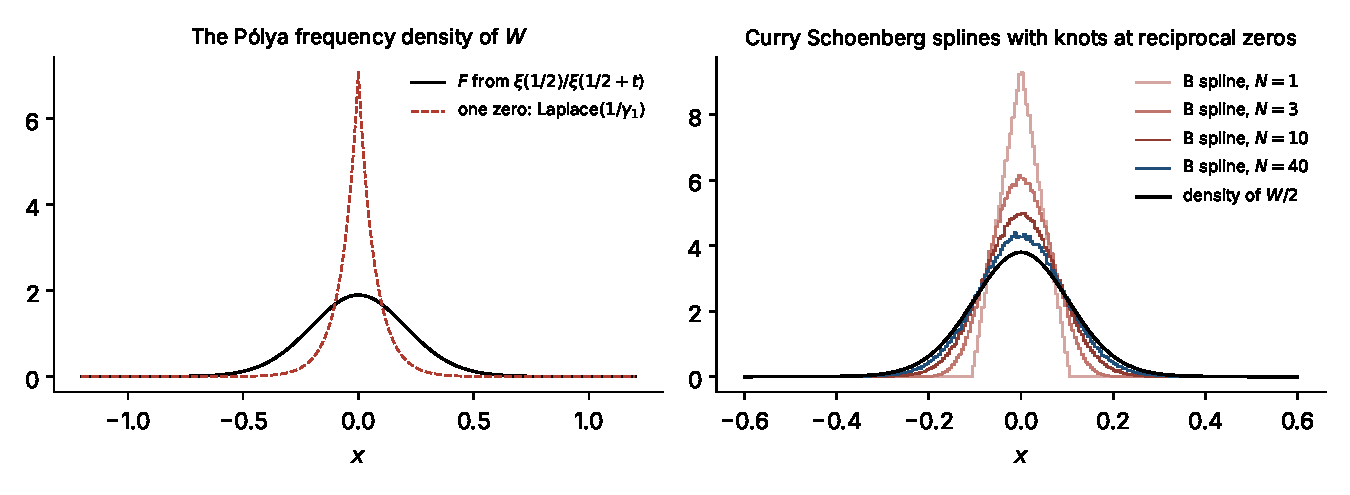
\includegraphics[width=\textwidth]{fig/v3/fig_pf_spline.pdf}
\caption{Left: the P\'olya frequency density of $W$ from $\xi(\frac12)/\xi(\frac12+t)$, with the Laplace density of the first zero alone for comparison. Right: B splines with knots $0,\pm\frac{2N+1}{2\gamma_n}$ converge to the density of $W/2$ (simulation, computed).}
\label{g:fig:pf}
\end{figure}
% UNVERIFIED: the figure was not redrawn by the referees; its simulated curves are illustrations only (V3C: the Monte Carlo grids are not reproducible); the sup errors printed in the draft are omitted.

\section{Splines inside the sine squared lemma}\label{g:sec:splinelemma}

The kernel of the sine squared lemma \eqref{eq:sin2} is the Fourier transform of the hat B spline $H(y)=(1-|y|)_+$. In the book's chart ($u=w^2$, $z=\theta^2$), the density of the lemma is
\[
\frac{\tau_x(z)}{x}=\frac{\sin^2(x\sqrt z/2)}{\pi\sqrt z}=\frac{x^2\sqrt z}{4\pi}\,\widehat H(x\sqrt z),\qquad\widehat H(\theta)=\Big(\frac{\sin(\theta/2)}{\theta/2}\Big)^2\ge0 .
\]
Positivity of the transfer from L\'evy to Thorin measures is positivity of the Fourier transform of a B spline, the Fej\'er kernel. The centred B spline $B_{2m}$ of order $2m$ (the $2m$ fold convolution of the indicator of $[-\frac12,\frac12]$) has $\widehat B_{2m}(\theta)=(\sin(\theta/2)/(\theta/2))^{2m}\ge0$, and it gives the following family.

\begin{theorem}[Spline lemma]\label{g:thm:splinelemma}
Let $m\ge1$, $x,w>0$, and
\[
a_j=\frac{2(-1)^{j+1}}{j}\binom{2m}{m+j}\qquad(1\le j\le m).
\]
Then
\begin{gather}
\sum_{j=1}^ma_j\big(e^{-jwx}-1+jwx\big)=\int_0^\infty\log\Big(1+\frac{w^2}z\Big)\tau^{(m)}_x(z)\,\mathrm dz,\label{g:eq:splinelemma}\\
\tau^{(m)}_x(z)=\frac x{2\pi}\,\frac{\big(2\sin(x\sqrt{z}/2)\big)^{2m}}{\sqrt{z}}\ge0 .\notag
\end{gather}
\end{theorem}

\begin{proof}
Substitute $z=y^2$, so the right side is $\frac x\pi\int_0^\infty\log(1+w^2/y^2)\,(2\sin(xy/2))^{2m}\mathrm dy$. Expand
\[
\Big(2\sin\frac\theta2\Big)^{2m}=\binom{2m}{m}+2\sum_{j=1}^m(-1)^j\binom{2m}{m+j}\cos(j\theta)
\]
and use
\begin{gather*}
\int_0^\infty\log\Big(1+\frac{w^2}{y^2}\Big)\mathrm dy=\pi w,\\
\int_0^\infty\log\Big(1+\frac{w^2}{y^2}\Big)\cos(jxy)\,\mathrm dy=\frac{\pi(1-e^{-jwx})}{jx}
\end{gather*}
(the second is integration by parts and the integral used to prove the sine squared lemma). The right side becomes $\binom{2m}{m}wx+2\sum_j(-1)^j\binom{2m}{m+j}\frac{1-e^{-jwx}}{j}$. Since $\binom{2m}{m}+2\sum_{j\ge1}(-1)^j\binom{2m}{m+j}=0$, the linear term equals $-2\sum_j(-1)^j\binom{2m}{m+j}\frac{jwx}{j}$, and collecting terms gives the left side.
\end{proof}

For $m=1$, $a_1=2$ and \eqref{g:eq:splinelemma} is twice the sine squared lemma. For $m=2$ the weights are $(8,-1)$, and for $m=3$ they are $(30,-6,\frac23)$.
\begin{corollary}\label{g:cor:spline}
Let $\kappa_m\ge0$ be measures on $(0,\infty)$ and $\nu_+\ge0$. Every L\'evy measure of the form
\[
\nu=\nu_++\sum_{m\ge1}\int_0^\infty\sum_{j=1}^ma^{(m)}_j\,\delta_{jx}\,\kappa_m(\mathrm dx),
\]
with the integrability that makes the Fubini exchange and the full compensation absolutely convergent, has a positive Thorin image in the variable $u=w^2$, even though $\nu$ may be signed.
\end{corollary}

\begin{proof}
The transfer is linear; apply the sine squared lemma to $\nu_+$ and Theorem~\ref{g:thm:splinelemma} to each pattern.
\end{proof}

Nakamura's measure lives on the prime power lattices $\log p\,\mathbb N$ plus smooth parts, which is the geometry of the spline patterns: a pattern $\sum_ja_j\delta_{jx}$ with $x=\log p$ sits on the powers of $p$. The positivity of Thorin densities from signed canonical measures is not new in the book (it is in Section~\ref{ch:basepoint}, where $x\Pi_1$ is negative beyond $x=0.28120$, and in Proposition~\ref{dl:prop:hecke2sin} for signed Hecke weights); the spline lemma adds the family of patterns. The spline lemma is, as far as we know, not in the literature; we have not searched for it systematically. It comes from an unrefereed note of Polson (November 2026).

\section{All lattice patterns: the Fej\'er Riesz theorem}\label{g:sec:fr}

The spline patterns are not the only signed lattice measures with positive Thorin image. The classification is Theorem~\ref{g:thm:fr} below, built on the classical Fej\'er Riesz lemma; the analogue for Hecke weights is Theorem~\ref{dl:thm:cone}.

\begin{theorem}\label{g:thm:fr}
Let $h>0$ and $b_1,\dots,b_n\in\mathbb R$, and let $\nu=\sum_{j=1}^nb_j\delta_{jh}$ be a fully compensated L\'evy measure. Its Thorin image under the transfer of the sine squared lemma has density, in the variable $z=\theta^2$,
\[
\frac{h}{2\pi\theta}\,T(\theta h),\qquad T(\vartheta)=\sum_{j=1}^n j\,b_j\,\big(1-\cos j\vartheta\big),
\]
so it is positive if and only if $T\ge0$. By the Fej\'er Riesz theorem this holds if and only if
\[
T(\vartheta)=\big|(1-e^{i\vartheta})\,q(e^{i\vartheta})\big|^2
\]
for a polynomial $q$ with real coefficients and degree at most $n-1$.
\end{theorem}

\begin{proof}
By the sine squared lemma a compensated atom of mass $b$ at $y$ has Thorin density $b\,y\,\sin^2(\theta y/2)/(\pi\theta)=b\,y(1-\cos\theta y)/(2\pi\theta)$ in $z=\theta^2$ (equation~\eqref{eq:sin2} with $z=\theta^2$ in the density); summing over $y=jh$ gives the formula. A nonnegative cosine polynomial $T$ of degree $n$ is $|p(e^{i\vartheta})|^2$ with $p$ real of degree $n$ (Fej\'er Riesz). Since $T(0)=0$, $p(1)=0$ and $p(z)=(1-z)q(z)$. The map from $(b_j)$ to $T$ is a bijection onto the cosine polynomials of degree $n$ vanishing at $0$.
\end{proof}

The spline lemma is the case $q(z)=(1-z)^{m-1}$, for which $T(\vartheta)=(2\sin\frac\vartheta2)^{2m}$ up to a constant. Every other nonnegative cosine polynomial vanishing at the origin gives another pattern, and these are all of them: the cone of signed lattice measures with positive Thorin image on a single lattice is generated by the Fej\'er Riesz squares $|(1-z)q(z)|^2$.

\begin{remark}[The same mechanism in the zero free region]\label{g:rem:dvp}
For $\sigma>1$ and any nonnegative cosine polynomial $T(\vartheta)=\sum_jc_j\cos j\vartheta$, the nonnegativity of $\Lambda(n)$ gives
\[
\sum_jc_j\,\Re\Big(-\frac{\zeta'}{\zeta}\Big)(\sigma+ijt)=\sum_n\Lambda(n)n^{-\sigma}\,T(t\log n)\ \ge\ 0 .
\]
With $T(\vartheta)=3+4\cos\vartheta+\cos2\vartheta=\frac12|1+e^{i\vartheta}|^4=2(1+\cos\vartheta)^2$ this is de la Vall\'ee Poussin's inequality. Its Thorin form is Proposition~\ref{tx3:prop:dvp}, and the optimisation over higher degree squares is in Section~\ref{cf:sec:arith}. In the language of this chapter, de la Vall\'ee Poussin applies a Fej\'er Riesz square on the prime lattices, while Thorin positivity applies the square $|1-e^{i\vartheta}|^2$ to the full measure $\mu$.
\end{remark}

\section{The strip form: the pole changes sides}\label{g:sec:strip}

Inside the critical strip the ledger rearranges itself. Write $k_\sigma$ for the compensated density \eqref{n:eq:k} of Chapter~\ref{n:ch:nakamura}, $\pi k_\sigma(v)=\Re\frac{\xi'}{\xi}(\sigma+iv)-\frac{\xi'}{\xi}(\sigma)$. The uncompensated density $\frac1\pi\Re\frac{\xi'}{\xi}(\sigma+iv)$ is the one of Theorem~\ref{sm:thm:strip}; the two differ by the drift $\frac1\pi\frac{\xi'}{\xi}(\sigma)$, which is positive for $\sigma>\frac12$.

\begin{theorem}\label{g:thm:strip}
For $\frac12<\sigma<1$ and $v>0$, away from the ordinates,
\[
\pi k_\sigma(v)=\underbrace{\Re\frac{\zeta'}{\zeta}(\sigma+iv)-\frac{\zeta'}{\zeta}(\sigma)}_{P^{\rm reg}_\sigma(v)}\;+\;\underbrace{A_\sigma(v)}_{\ge0}\;+\;\underbrace{\frac{v^2}{(1-\sigma)\big((1-\sigma)^2+v^2\big)}}_{B_\sigma(v)\,\ge0},
\]
with $A_\sigma(v)=\frac12[\Re\psi(\frac{\sigma+iv}2)-\psi(\frac\sigma2)]-\frac{v^2}{\sigma(\sigma^2+v^2)}\ge0$. Hence $k_\sigma\ge0$ for every $\sigma\in(\frac12,1)$ if and only if, for every $\sigma\in(\frac12,1)$ and every $v$ that is not an ordinate of a pole of $\zeta'/\zeta$,
\begin{equation}\label{g:eq:stripineq}
\Re\frac{\zeta'}{\zeta}(\sigma+iv)\ \ge\ \frac{\zeta'}{\zeta}(\sigma)-A_\sigma(v)-B_\sigma(v).
\end{equation}
By Theorem~\ref{cx:thm:rhmin} this holds if and only if RH holds, and the direction that RH gives $k_\sigma\ge0$ is a consequence of that theorem (it needs the minimum over $v$ of the compensated density to sit at $v=0$).
\end{theorem}

\begin{proof}
Take real parts in $\frac{\xi'}{\xi}(s)=\frac1s+\frac1{s-1}-\frac12\log\pi+\frac12\psi(\frac s2)+\frac{\zeta'}{\zeta}(s)$ at $s=\sigma+iv$ and subtract the value at $s=\sigma$. The pole term gives $\Re\frac1{s-1}-\frac1{\sigma-1}=\frac{v^2}{(1-\sigma)((1-\sigma)^2+v^2)}$, which is positive for $\sigma<1$. $A_\sigma\ge0$ because it is the $(1-\cos)$ transform of the positive density $e^{-\sigma x}/(e^{2x}-1)$, convergent for $\sigma>-2$. The equivalence is Theorem~\ref{cx:thm:rhmin}.
\end{proof}

For $\sigma>1$ the primes are the friend and the pole is the enemy: the prime term is nonnegative and the pole term is subtracted. Inside the strip the roles reverse. The pole and the gamma factor both contribute nonnegative terms, and the only term that can be negative is the analytically continued prime term $P^{\rm reg}_\sigma$.

\begin{table}[t]
\centering
\footnotesize
\begin{tabular}{lccccc}
\toprule
$\sigma$ & $P^{\rm reg}<0$ & worst ratio & at $v$ & $P^{\rm reg}$ & $A+B$\\
\midrule
0.55 & 91\% & 0.9973 & 17.49 & $-3.396$ & 3.406\\
0.75 & 100\% & 0.9911 & 17.49 & $-5.084$ & 5.129\\
0.90 & 100\% & 0.9935 & 17.49 & $-11.020$ & 11.092\\
\bottomrule
\end{tabular}
\caption{How much room inequality \eqref{g:eq:stripineq} leaves on $14\le v\le300$ (computed on a grid). The second column is the share of grid points where the continued prime term is negative; the third is the worst ratio $-P^{\rm reg}/(A+B)$ on the grid. The values at $v=17.49$ were reproduced independently; the grid point is not the continuous optimiser.}
\label{g:tab:strip}
\end{table}
% UNVERIFIED: the percentages of the second column and the extrema over the whole grid were not reproduced (V3C: grid and interpolation not specified); the point values at v=17.49 were.

Table~\ref{g:tab:strip} shows that the inequality has little room where it matters: on the grid the continued prime term is negative at most sampled points, and at its worst it uses more than $99\%$ of what the gamma factor and the pole provide, in the first gap between zeros, where the margin is below one percent. Any proof of \eqref{g:eq:stripineq} must be sharp to that extent.

\section{Equivalent forms of RH, and what the ledger leaves}\label{g:sec:chain}

\begin{remark}[Six forms]\label{g:rem:chain}
The following statements are equivalent to RH, by the results cited. (1) $k_\sigma\ge0$ for every $\sigma\in(\frac12,1)$, that is \eqref{g:eq:stripineq} (Theorem~\ref{g:thm:strip}). (2) Nakamura: the characteristic function $\Xi_\sigma$ is pretended infinitely divisible for every $\sigma\in(\frac12,1)$ (Theorem~\ref{n:thm:nak}, \cite{Nakamura15}). (3) Carath\'eodory: $\Re\frac{\xi'}{\xi}(s)>0$ on $\Re s>\frac12$, which is Lagarias's positivity property \cite{Lagarias}. The reasons are that $\frac{\xi'}{\xi}(\sigma)>0$ for $\sigma>\frac12$ unconditionally (pair $\rho$ with $1-\bar\rho$) and $\Re\frac{\xi'}{\xi}\to-\infty$ just left of a zero off the line. (4) Weil's criterion in Bombieri's form, positivity of Weil's quadratic form on test functions (Weil and Bombieri \cite{Bombieri}; the form in Theorem~\ref{wt:thm:main} is the heat form). % TODO: define the regularised distribution D(h) with the constant at h(0) and the Fourier convention (2 pi factor), or keep the citation only.
 (5) Schoenberg: the density with characteristic function $\xi(\frac12)/\xi(\frac12+t)$ is a P\'olya frequency function (Proposition~\ref{pol:prop:pf}). (6) The B spline knots $\pm\frac{2N+1}{2\gamma_n}$ are real for every ordinate $\gamma_n$ (all zeros enumerated), which restates RH directly (knots real if and only if ordinates real; compare Proposition~\ref{g:prop:bspline}) and adds nothing to it. None of the moves between these coordinate systems is a proof: a proof must establish one item from information that does not already contain the zeros.
\end{remark}

In the EGGC density, $\pi k_\sigma=P_\sigma+A_\sigma-R_\sigma$, with $P_\sigma$ from the primes, $A_\sigma$ from the gamma factor and $R_\sigma$ from the pole. The ledger explains each piece. $A_\sigma\ge0$ is the gamma factor after the factor $s$ has removed its first pole; it comes from $\sum_{k\ge1}e^{-2kx}$ and grows like $\frac12\log v$, controlling large frequencies. For $\sigma>1$, where $P_\sigma$ is a prime sum, $R_\sigma$ is the pole, bounded by $1/(\sigma-1)$, and the primes must beat it at small and moderate frequencies, which is the third cancellation of Remark~\ref{g:rem:four}. The first two cancellations are exact, so the gamma factor's share of the ledger is settled and RH concerns the third and the remainder.

\section{Three programmes}\label{g:sec:pathgp}

Remark~\ref{g:rem:chain} says what a path must do: prove one of its items from data that do not already encode the zeros. Three items are stated in such data. Item (1) in the form \eqref{g:eq:stripineq} involves only $\zeta'/\zeta$ in the strip, the gamma function and the pole. Item (4) involves only the prime measure, the density $e^x$ and the gamma density. Item (5) involves only $\xi$ on the real axis, computed from the Dirichlet eta series and the gamma function. These are programmes A, B and C. They are heuristic assessments, not results.

\paragraph{Programme A: positivity certificates (items 1 and 4).} Write the inequality as a nonnegative combination of manifestly nonnegative pieces. For $\sigma>1$ Thorin positivity holds (Proposition~\ref{bp:prop:valpha}), and the Fej\'er Riesz square $2(1+\cos\vartheta)^2$ on the prime lattices gives de la Vall\'ee Poussin's zero free region (Remark~\ref{g:rem:dvp}). The obstruction inside the strip is regularisation. The prime sum $\sum\Lambda(n)n^{-\sigma}(1-\cos(v\log n))$ diverges for $\sigma<1$, and the convergent object is its analytic continuation $P^{\rm reg}_\sigma$, which Table~\ref{g:tab:strip} shows is negative at most grid points. Regularisation does not preserve positivity, as $\sum n=-\frac1{12}$ shows. What is missing is a positivity principle for regularised sums: conditions on a positive sequence under which the regularised value of a nonnegative trigonometric combination stays above a prescribed negative bound, here the bound $-A_\sigma-B_\sigma$ of Theorem~\ref{g:thm:strip} met with less than one percent to spare (Table~\ref{g:tab:strip}).

\paragraph{Programme B: descent (items 3 and 4).} $\frac{\xi'}{\xi}$ is a Carath\'eodory function on $\Re s>1$ unconditionally. Moving the line from $\sigma$ to $\sigma-\varepsilon$ multiplies the Fourier transform of the boundary density by $e^{\varepsilon|x|}$, and positivity survives exactly when $e^{\varepsilon|x|}e^{-\sigma|x|}\mu(\mathrm d|x|)$ stays of the positive type of item (4). % TODO: state the precise positive definiteness with the constant $c_\sigma$ when $k_\sigma$ is the target.
 Every rung of this ladder below $\sigma=1$ asserts a zero free half plane, so each is a quasi Riemann hypothesis, a theorem above $\frac78$ by \cite{OAI26a} and open below. What is missing is control of the growth of the prime remainder's Fourier transform under the exponential weight, which is the explicit formula read backwards.

\paragraph{Programme C: total positivity (item 5).} This programme is the Pólya frequency ladder of Proposition~\ref{pol:prop:pf} and Problem~\ref{pol:op:pf2}, with the floating point certificate of PF$_2$ in Theorem~\ref{pol:thm:pf2}. A proof of PF$_k$ for all $k$ is RH. The authors do not claim that any rung beyond the numerical evidence has been proved.

\section{Open problems}\label{g:sec:open}

Log concavity of the density $f_X$ and the higher rungs of the ladder are Problem~\ref{pol:op:pf2}. The following problems are specific to this chapter.

\begin{enumerate}
\item A positivity principle for regularised sums. Find conditions on a nonnegative sequence $c_n$ and a nonnegative trigonometric weight under which the regularised sum $\sum c_nn^{-\sigma}T(v\log n)$ for $\sigma<1$ is bounded below by an explicit negative quantity. The target is \eqref{g:eq:stripineq}, with less than one percent room.
\item Fej\'er Riesz on several lattices. Theorem~\ref{g:thm:fr} classifies patterns on one lattice. The primes give the independent lattices $\log p\,\mathbb N$, and by Bohr's correspondence the prime part becomes a function on an infinite torus, where nonnegative trigonometric polynomials need not be sums of squares (Hilbert, Rudin). Determine which sum of squares certificates on the Bohr torus survive the regularisation of problem 1.
\item The tight gap. Explain analytically why, on $v\ge14$, \eqref{g:eq:stripineq} is tightest near $v\approx17.5$, inside the gap $(\gamma_1,\gamma_2)$, and bound the margin there in terms of the gap length.
\end{enumerate}
